

\tikzset{every picture/.style={line width=0.75pt}} %set default line width to 0.75pt        

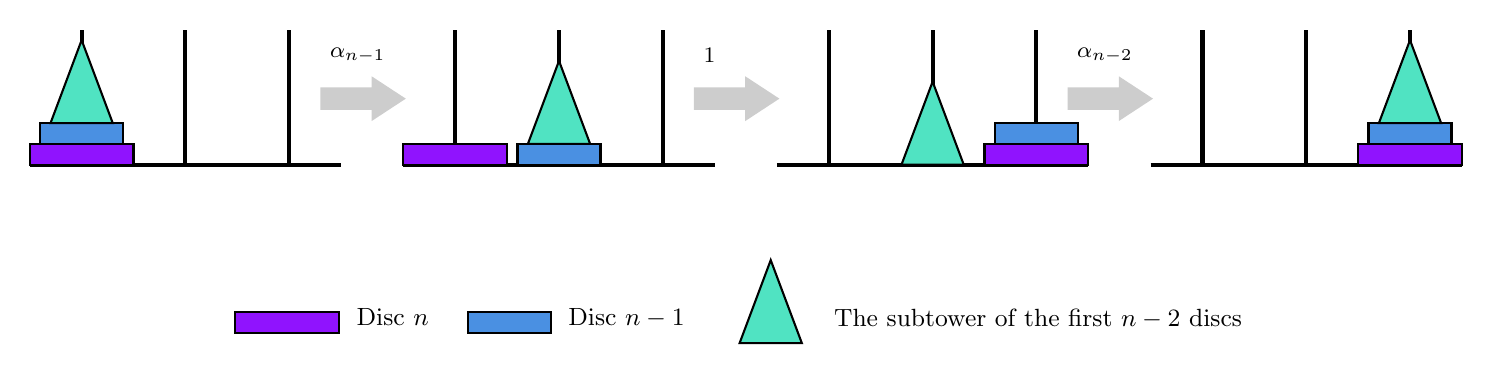
\begin{tikzpicture}[x=0.75pt,y=0.75pt,yscale=-1,xscale=1]
%uncomment if require: \path (0,241); %set diagram left start at 0, and has height of 241

%Straight Lines [id:da24815424100458983] 
\draw [line width=1.5]    (75,65) -- (75,0) ;
%Straight Lines [id:da8115465333076248] 
\draw [line width=1.5]    (125,65) -- (125,0) ;
%Straight Lines [id:da9739766763946329] 
\draw [line width=1.5]    (25,65) -- (25,0) ;
%Straight Lines [id:da6210476839521044] 
\draw [line width=1.5]    (0,65) -- (150,65) ;
%Shape: Rectangle [id:dp9225038130009493] 
\draw  [fill={rgb, 255:red, 74; green, 144; blue, 226 }  ,fill opacity=1 ] (5,45) -- (45,45) -- (45,55) -- (5,55) -- cycle ;
%Shape: Rectangle [id:dp9657809601082321] 
\draw  [fill={rgb, 255:red, 144; green, 19; blue, 254 }  ,fill opacity=1 ] (0,55) -- (50,55) -- (50,65) -- (0,65) -- cycle ;
%Shape: Triangle [id:dp7994638232866984] 
\draw  [fill={rgb, 255:red, 80; green, 227; blue, 194 }  ,fill opacity=1 ] (25,5) -- (40,45) -- (10,45) -- cycle ;
%Straight Lines [id:da6351702401045551] 
\draw [line width=1.5]    (255,65) -- (255,0) ;
%Straight Lines [id:da23539284354694123] 
\draw [line width=1.5]    (305,65) -- (305,0) ;
%Straight Lines [id:da6407367265186239] 
\draw [line width=1.5]    (205,65) -- (205,0) ;
%Straight Lines [id:da8823485940887543] 
\draw [line width=1.5]    (180,65) -- (330,65) ;
%Shape: Rectangle [id:dp7145285546098397] 
\draw  [fill={rgb, 255:red, 74; green, 144; blue, 226 }  ,fill opacity=1 ] (235,55) -- (275,55) -- (275,65) -- (235,65) -- cycle ;
%Shape: Rectangle [id:dp11686590820323883] 
\draw  [fill={rgb, 255:red, 144; green, 19; blue, 254 }  ,fill opacity=1 ] (180,55) -- (230,55) -- (230,65) -- (180,65) -- cycle ;
%Shape: Triangle [id:dp326144810998521] 
\draw  [fill={rgb, 255:red, 80; green, 227; blue, 194 }  ,fill opacity=1 ] (255,15) -- (270,55) -- (240,55) -- cycle ;
%Straight Lines [id:da38727899106831454] 
\draw [line width=1.5]    (435,65) -- (435,0) ;
%Straight Lines [id:da4098652212962761] 
\draw [line width=1.5]    (485,65) -- (485,0) ;
%Straight Lines [id:da6850068143481041] 
\draw [line width=1.5]    (385,65) -- (385,0) ;
%Straight Lines [id:da8948080700978496] 
\draw [line width=1.5]    (360,65) -- (510,65) ;
%Shape: Rectangle [id:dp7946080570799627] 
\draw  [fill={rgb, 255:red, 74; green, 144; blue, 226 }  ,fill opacity=1 ] (465,45) -- (505,45) -- (505,55) -- (465,55) -- cycle ;
%Shape: Rectangle [id:dp5580963644428822] 
\draw  [fill={rgb, 255:red, 144; green, 19; blue, 254 }  ,fill opacity=1 ] (460,55) -- (510,55) -- (510,65) -- (460,65) -- cycle ;
%Shape: Triangle [id:dp20454638540295167] 
\draw  [fill={rgb, 255:red, 80; green, 227; blue, 194 }  ,fill opacity=1 ] (435,25) -- (450,65) -- (420,65) -- cycle ;
%Straight Lines [id:da71545551051053] 
\draw [line width=1.5]    (615,65) -- (615,0) ;
%Straight Lines [id:da42952519976526493] 
\draw [line width=1.5]    (665,65) -- (665,0) ;
%Straight Lines [id:da02676389926063205] 
\draw [line width=1.5]    (565,65) -- (565,0) ;
%Straight Lines [id:da513368833927792] 
\draw [line width=1.5]    (540,65) -- (690,65) ;
%Shape: Rectangle [id:dp9163905899859819] 
\draw  [fill={rgb, 255:red, 74; green, 144; blue, 226 }  ,fill opacity=1 ] (645,45) -- (685,45) -- (685,55) -- (645,55) -- cycle ;
%Shape: Rectangle [id:dp23350695623157525] 
\draw  [fill={rgb, 255:red, 144; green, 19; blue, 254 }  ,fill opacity=1 ] (640,55) -- (690,55) -- (690,65) -- (640,65) -- cycle ;
%Shape: Triangle [id:dp5086883694866662] 
\draw  [fill={rgb, 255:red, 80; green, 227; blue, 194 }  ,fill opacity=1 ] (665,5) -- (680,45) -- (650,45) -- cycle ;
%Right Arrow [id:dp02688709887459506] 
\draw  [draw opacity=0][fill={rgb, 255:red, 155; green, 155; blue, 155 }  ,fill opacity=0.5 ] (140,27.81) -- (164.71,27.81) -- (164.71,22.41) -- (181.18,33.2) -- (164.71,44) -- (164.71,38.6) -- (140,38.6) -- cycle ;
%Right Arrow [id:dp7559893443766514] 
\draw  [draw opacity=0][fill={rgb, 255:red, 155; green, 155; blue, 155 }  ,fill opacity=0.5 ] (320,27.81) -- (344.71,27.81) -- (344.71,22.41) -- (361.18,33.2) -- (344.71,44) -- (344.71,38.6) -- (320,38.6) -- cycle ;
%Right Arrow [id:dp6938789629236952] 
\draw  [draw opacity=0][fill={rgb, 255:red, 155; green, 155; blue, 155 }  ,fill opacity=0.5 ] (500,27.81) -- (524.71,27.81) -- (524.71,22.41) -- (541.18,33.2) -- (524.71,44) -- (524.71,38.6) -- (500,38.6) -- cycle ;
%Shape: Rectangle [id:dp8166502832119333] 
\draw  [fill={rgb, 255:red, 144; green, 19; blue, 254 }  ,fill opacity=1 ] (99,136) -- (149,136) -- (149,146) -- (99,146) -- cycle ;

%Shape: Rectangle [id:dp6910609554250948] 
\draw  [fill={rgb, 255:red, 74; green, 144; blue, 226 }  ,fill opacity=1 ] (211,136) -- (251,136) -- (251,146) -- (211,146) -- cycle ;

%Shape: Triangle [id:dp018656944685809806] 
\draw  [fill={rgb, 255:red, 80; green, 227; blue, 194 }  ,fill opacity=1 ] (357,111) -- (372,151) -- (342,151) -- cycle ;


% Text Node
\draw (143.18,7.4) node [anchor=north west][inner sep=0.75pt]  [font=\footnotesize]  {$\alpha_{n-1}$};
% Text Node
\draw (323.18,7.4) node [anchor=north west][inner sep=0.75pt]  [font=\footnotesize]  {$1$};
% Text Node
\draw (503.18,7.4) node [anchor=north west][inner sep=0.75pt]  [font=\footnotesize]  {$\alpha_{n-2}$};
% Text Node
\draw (258,133) node [anchor=north west][inner sep=0.75pt]  [font=\small] [align=left] {Disc $\displaystyle n-1$};
% Text Node
\draw (156,133) node [anchor=north west][inner sep=0.75pt]  [font=\small] [align=left] {Disc $\displaystyle n$};
% Text Node
\draw (386,133) node [anchor=north west][inner sep=0.75pt]  [font=\small] [align=left] {The subtower of the first $\displaystyle n-2$ discs};


\end{tikzpicture}